\chapter[Desenvolvimento do Sistema]{Desenvolvimento do Sistema}
%---------------------------------------------------------------------------
\section{Processo de Desenvolvimento}
%<Neste item deve ser descrito de forma detalhada o proecsso de desenvolvimento que foi utilizado definindo as etapas deste processo>

O desenvolvimento se iniciou a partir do módulo de scraping feito em python, foram feitos scripts iniciais que serviram de prova de conceito para a execução das tarefas de scraping do site da prefeitura de Uberlândia. Após a criação dos primeiros scripts e a obtenção dos documentos se mostrar possível, foi realizada a estruturação da base de dados SQLite que serve como base de busca textual.

Desta forma, com os documentos obtidos através das primeiras versões dos scripts python de scraping e a versão inicial do banco de dados, foram criados os primeiros scripts que fazem a extração do conteúdo textual dos documentos e armazena no banco de dados. O que já permitiu a realização de consultas textuais a partir do módulo de full text search do SQLite.

A parte final do desenvolvimento do módulo de scraping se resumiu em refinar e organizar os scripts que até aqui atuavam separadamente de forma a trabalharem em conjunto em um fluxo que permitisse uma execução única e mais automatizada.

Com isto, foi construída uma base para que os outros dois módulos pudessem operar, com a estrutura de banco de dados definida e o módulo de scraping e indexação já funcionando para obter um conjunto inicial de documentos a partir do site da prefeitura de Uberlândia foi possível iniciar a construção da API que fica responsável por consumir a base de dados indexada.

O desenvolvimento da API, assim como da aplicação web de frontend foi executado em menor tempo devido a maior familiaridade com as tecnologias escolhidas, além de que com a estruturação feita durante o desenvolvimento do módulo de indexação foi possível agilizar o desenvolvimento de ambas as ferramentas. Após a conclusão das versões iniciais já funcionais foi realizado algumas etapas de refinamento de código em todos os módulos para correções de bugs e melhorias nas estruturas de projeto e funcionamento geral do sistema.
%---------------------------------------------------------------------------
\section{Arquitetura do Sistema}
O sistema foi desenvolvido utilizando uma arquitetura cliente-servidor de três camadas, composta pela camada de apresentação, camada de serviços e camada de dados. Essa separação permite a organização de responsabilidades entre os componentes do sistema, que possui camadas bem definidas que interoperam.

A camada de apresentação é composta por uma aplicação web desenvolvida usando React e Vite, ela é responsável pela interação do usuário através de uma interface gráfica e seu acesso é feito através de um navegador web.

A camada de serviços é constituída por uma API REST desenvolvida em .NET 9, responsável pelo processamento de requisições vindas da aplicação web, aplicação de regras de negócio e acesso aos dados armazenados. A API disponibiliza endpoints para pesquisa textual, recuperação de diários por id e obtenção de documentos mais recentes.

Já a camada de dados utiliza o banco SQLite que é responsável por armazenar os dados extraídos dos documentos dos Diários Oficiais Municipais, o sistema foi construído de forma que cada cidade indexada possui uma instância de banco sqlite separada, quando uma requisição é feita para buscas de documentos a API recebe por parâmetro qual cidade deve ser acessada, o mesmo ocorre durante o processo de indexação. No caso deste trabalho apenas a cidade de Uberlândia foi utilizada no desenvolvimento, por isso ela é a única presente como possibilidade de seleção no módulo de frontend no estado atual do sistema.

O processo de coleta e indexação é realizado por um web scraper desenvolvido em Python. O módulo de scraping também se limita ao script para o site da prefeitura de Uberlândia em seu estagio atual, mas seu desenvolvimento foi pensado de forma modular para possibilitar a adição de scripts de scraping para os sites de outras prefeituras. O scraper é executado de forma automatizada ou manualmente através de linha de comando e pode buscar arquivos na web ou indexar arquivos que já estejam salvos localmente.

Durante o desenvolvimento, a infraestrutura da aplicação foi implantada em um servidor Ubuntu Server. A API .NET e um servidor web Nginx foram executados em contêineres Docker gerenciados pelo Docker Compose, enquanto o web scraper é executado diretamente no sistema operacional do servidor. O banco de dados SQLite também permanece no sistema de arquivos do próprio servidor e é compartilhado entre a API por meio de um diretório montado como volume no contêiner da API.

O servidor Nginx é responsável por disponibilizar os arquivos estáticos gerados na construção da aplicação React e também por atuar como proxy reverso recebendo as requisições destinadas para a API. O acesso externo é feito através do Cloudflare Tunnel, que estabelece uma conexão segura entre o servidor e a infraestrutura da Cloudflare, permitindo que o serviço seja acessado na web e elimina a necessidade de exposição direta de portas na rede.

Como requisitos mínimos de infraestrutura para execução do sistema, usando como base a infraestrutura usada durante o desenvolvimento, recomenda-se um servidor com sistema operacional Linux, processador de dois núcleos, 2 GB de memória RAM e aproximadamente 5 GB de espaço livre em disco para armazenamento da aplicação e do banco de dados, além do acesso a internet.

%<Neste item deve ser apresentada a arquitetura de infra-estrutura do sistema, demonstrando o tipo de arquitetura que será utilizada (por exemplo, cliente/servidor de n-camadas), a configuração de hardware, de rede e de software a serem utilizados, bem como o dimensionamento mínimo de conexões.>

\section{Tecnologias Utilizadas no Desenvolvimento}

A escolha das ferramentas para desenvolvimento do sistema foi focada na facilidade que cada ferramenta oferece para atingir o objetivo de operação de cada camada, além da familiaridade do autor com as mesmas. 

No caso da camada de scraping e indexação (dados), o desenvolvimento foi feito usando Python 3.14, sendo as três principais bibliotecas utilizadas, a "pypdf", para leitura e extração textual dos documentos, a "Requests", para obtenção das páginas web, e a "BeaultifulSoup", para \textit{parsing} dos html obtidos. Além delas foram utilizadas bibliotecas padrão da linguagem, que contém ferramentas para trabalho com diretórios, arquivos e também acesso ao banco de dados SQLite.

Já na camada de backend (serviços), foi utilizado o framework .NET Core 9, usando linguagem C\#, com as principais bibliotecas utilizadas além da biblioteca padrão do framework sendo a "Microsoft.Data.Sqlite", para conexão com a base de dados, "Serilog", para geração de logs, "Scalar", para geração de documentação da API e as bibliotecas "Moq" e "xunit", que são utilizadas nos testes unitários.

Na camada de frontend (apresentação), foi utilizado Typescript através do ReactJs em conjunto com a ferramenta de construção vite para criação da interface de usuário web. Foram usadas duas bibliotecas principais, sendo elas a "tanstack/react-query" para gerenciamento de dados e a "zustand" para gerenciamento de estados.

O banco de dados SQLite é a ferramenta central, já que o recurso de FTS (Full Text Search) do próprio SQLite é o que permite a busca textual dos arquivos nele indexados. A utilização da ferramenta é bastante facilitada por não exigir instalação de nenhuma ferramenta/ambiente para criação e/ou gerenciamento da base de dados, este trabalho pode ser feito diretamente a partir do código das aplicações que utilizam o SQLite como persistência de dados. Outra vantagem é que o espaço de armazenamento é bastante reduzido, o banco existe em apenas um arquivo ".db" que consome pouco espaço em disco mesmo após a inserção de dados. Para exemplificação, durante os testes realizados em desenvolvimento, o espaço ocupado pelos arquivos pdf dos diários oficiais obtidos a partir do site da prefeitura de Uberlândia correspondentes ao período de 01/06/2026 até 23/07/2026 foi de 84,9 MB, já o espaço ocupado pelo banco de dados (arquivo "udi.db") com o conteúdo textual dos documentos pdf já indexados ocupa apenas 14,6 MB.



%<Neste item devem ser apresentados os softwares de desenvolvimento (linguagem de programação, banco de dados, ferramentas, etc.), equipamentos de hardware e redes que sejam essenciais para o desenvolvimento do sistema, Frameworks, Bibliotecas, .>

\subsection{Linguagens de desenvolvimento}
%<Listar, definir referenciar e descrever as linguagens de desenvolvimento utilizadas.>
Para o desenvolvimento das aplicações que compõem o sistema foram utilizadas três linguagens de programação: Python, C\# e TypeScript.

\begin{table}[h]
    \centering
    \caption{Linguagens de desenvolvimento}
    \label{tab:tabela_linguagens_dsv}
    \begin{tabularx}{\textwidth}{l l X}
        \toprule
        Linguagem & Versão & Descrição \\
        \midrule
        Python & 3.14 &Linguagem de script de alto nível. Usada no módulo de scraping para obtenção e indexação dos documentos. \\
        C\# & 13.0 &Linguagem orientada a objetos pertencente ao ecossistema .NET. Usada no módulo de backend para desenvolvimento da API REST que serve ao frontend web. \\
        TypeScript & 6.0.2 &Linguagem de script que é uma extensão do JavaScript, adicionando tipagem. Usada no módulo de frontend para o desenvolvimento da pagina web de buscas. \\
        \bottomrule
    \end{tabularx}
\end{table}

As linguagens foram escolhidas levando em consideração dois fatores principais, sendo eles, o conhecimento prévio do autor no uso da linguagem e a facilidade de implementação dos recursos necessários em cada módulo. O objetivo foi facilitar ao máximo o desenvolvimento e manutenção dos diferentes módulos da aplicação.

A escolha do Python para o módulo de scraping se deu por ser uma linguagem interpretada e de fácil execução, com ampla quantidade de bibliotecas já existentes que facilitam o trabalho com requisições web (para obtenção dos documentos) e manipulação de arquivos (para leitura e indexação na base de dados), além de possuir o módulo de suporte ao banco de dados SQLite dentro da biblioteca padrão da linguagem.

No caso do módulo de backend, a familiaridade do autor com o ambiente .NET foi o principal fator de escolha, o que permitiu maior agilidade no desenvolvimento deste módulo. Por fim, no módulo de fronted, o TypeScript foi escolhido por ser uma ferramenta amplamente utilizada no contexto do desenvolvimento web moderno.

\section{Padrões de Projetos Utilizados}

No desenvolvimento do sistema foram utilizadas abordagens e padrões de projeto com o objetivo de organizar e facilitar a manutenção das aplicações envolvidas nos diferentes módulos, organizando a estrutura de código e separando responsabilidades. Os principais padrões utilizados estão relacionados à API do módulo backend, com separação de camadas, regras de negócio e acesso à base de dados.

O padrão Repository foi utilizado na camada de acesso aos dados, esta abordagem concentra as operações de leitura e manipulação do banco de dados em classes específicas, evitando que as outras camadas da aplicação tenham acesso direto aos mecanismos relacionados a persistência dos dados.

A aplicação também utiliza uma camada de serviços, operada por uma classe de serviço que é responsável por intermediar a comunicação entre os controladores (que são responsáveis pelas requisições) e a camada de repositório. Esta abordagem permite concentrar a aplicação das regras de operação em uma camada específica.

O padrão de Injeção de dependência é utilizado para controlar as dependências entre os componentes da API. Este padrão permite que as classes não precisem criar diretamente suas dependências, este trabalho é feito pelo mecanismo de injeção de dependência do ASP.NET Core.

Outro padrão utilizado foi o de uso de modelos de transferência de dados, que é a criação de modelos específicos para representar os dados recebidos e enviados pela API, separando as estruturas de requisição e resposta, além da entidade de dados dos diários. Permitindo o controle de quais informações são recebidas e disponibilizadas nos endpoints da aplicação.

Como já citado, a implementação faz uso do padrão de organização em camadas, separando as responsabilidades entre controllers, services e repositories. Os controladores são responsáveis pelo recebimento das requisições e retorno de respostas, a camada de serviço cuida das operações e regras do sistema e a camada de repositório do acesso aos dados. Esta organização permite reduzir o acoplamento entre partes da aplicação e facilita o desenvolvimento e manutenção, permitindo que uma camada seja modificada ou evolua de maneira independente.

%<Neste item devm ser descritos os padrões de projeto utilizados no desenvolvimento que soluções genéricas e comprovadas para problemas de design que surgem com frequência no desenvolvimento de software. Eles são descrições de alto nível de como resolver um problema específico, facilitando o desenvolvimento, a manutenção e a escalabilidade dos projetos.>

\subsection{Bibliotecas}

Para as bibliotecas utilizadas nas aplicações desenvolvidas, além das bibliotecas padrão de cada ferramenta utilizada para o desenvolvimento, algumas bibliotecas externas foram utilizadas para obtenção de melhores resultados.
Em todas as ferramentas desenvolvidas neste trabalho foram utilizadas bibliotecas auxiliares, as mais notáveis estão listadas na tabela X: 

\begin{table}[h]
    \centering
    \caption{Bibliotecas utilizadas}
    \label{tab:tabela_bibliotecas_utilizadas}
    \begin{tabularx}{\textwidth}{l l X}
        \toprule
        Ferramenta & Módulo & Função \\
        \midrule
        pypdf & Scraping &  Manipulação de arquivos PDF \\ 
        BeautifulSoup & Scraping &  Extração de dados de arquivos HTML \\ 
        Microsoft.Data.Sqlite & API Backend &  Interação com base de dados SQLite no sistema .NET \\
        Scalar & API Backend &  Criação de documentação interativa \\ 
        react-query & Frontend & Gerenciamento de estado assíncrono e busca de dados na API \\
        zustand & Frontend &   Gerenciamento de estado global de dados \\
        \bottomrule
    \end{tabularx}
\end{table}

%<Listar, definir referenciar e descrever as bibliotecas utilizadas no desenvolvimento.>
\subsection{Ferramentas Auxiliares}

As principais ferramentas auxiliares utilizadas foram o Visual Studio, que é uma IDE (Ambiente de Desenvolvimento Integrado)
voltada para o desenvolvimento de aplicações do ecossistema .NET, usada para o desenvolvimento da API do módulo de backend, e o Visual Studio Code, que é um editor de texto voltado para o desenvolvimento de software com capacidade para oferecer suporte a diferentes linguagens e ambientes de desenvolvimento, nele foram desenvolvidos os módulos de scraping e frontend.

Além dos editores, é possível listar também a ferramenta git, usada para o versionamento de código dos projetos.

%<Listar, definir referenciar e descrever as ferramentas auxiliares utilizadas no desenvolvimento.>

\subsection{Sistemas e componentes externos utilizados}

O uso de sistemas e componentes complementares ficou mais direcionado na implantação do sistema em um servidor próprio que foi utilizado durante o desenvolvimento. Dentre estes, os mais relevantes a serem citados são: Docker, Nginx, Ubuntu Server e Cloudflare Tunnels.

\begin{table}[h]
    \centering
    \caption{Sistemas e componentes externos}
    \label{tab:tabela_sistemas_e_componentes_externos}
    \begin{tabularx}{\textwidth}{l X}
        \toprule
        Componente & Descrição \\
        \midrule
        Docker & Plataforma utilizada para executar a API .NET e o servidor web Nginx em contêineres isolados \\
        Nginx & Servidor web responsável por disponibilizar os arquivos estáticos do frontend React e atuar como proxy reverso, encaminhando as requisições destinadas à API para o contêiner correspondente. \\
        Ubuntu Server & Sistema operacional do servidor utilizado para hospedar a aplicação, executar os contêineres Docker e disponibilizar o ambiente necessário para a execução do processo de coleta e indexação dos documentos. \\
        Cloudflare Tunnels & Serviço utilizado para estabelecer uma conexão segura entre o servidor de origem e a infraestrutura da Cloudflare, permitindo disponibilizar a aplicação externamente por meio de um domínio público sem exigir a exposição direta das portas do servidor à Internet. \\
        \bottomrule
    \end{tabularx}
\end{table}

%<Neste item devem ser descritos os sistemas e componentes externos que serão utilizados no sistema. Por exemplo, sistemas que serão integrados ao sistema desenvolvido, componentes comprados ou livre que estão sendo utilizados para facilitar ou complementar o desenvolvimento do sistema.>

%---------------------------------------------------------------------------
\section{Instalação e Configurações}

Nesta seção é descrita o processo de instalação e configuração das aplicações envolvidas no sistema de indexação e busca de diários, o sistema funciona como uma aplicação web e sua implementação é composta em três partes:

\begin{enumerate}
    \item Scraper em Python: responsável pela coleta e extração do conteúdo dos arquivos.
    \item API REST em .NET: responsável por disponibilizar os dados indexados e executar as consultas realizadas pelo frontend web.
    \item Frontend em React + TypeScript: responsável pela interface de busca e apresentação de resultados.
\end{enumerate}

A persistência dos dados é feita através do SQLite, com utilização do mecanismo SQLite FTS (Full-Text Search) para as consultas textuais. Durante o desenvolvimento, a aplicação foi hospedada em um servidor Ubuntu utilizando Docker para executar os componentes da API REST e o frontend React, já o scraper é executado diretamente no sistema operacional do servidor, onde um script de execução foi configurado para que o processo de busca e indexação aconteça de forma automatizada durante o período de testes da aplicação. Os componentes do sistema de busca possuem arquivos de configuração separados, durante a implantação se faz necessário ajustar estes arquivos de acordo com o ambiente em que o sistema está sendo executado, a principal razão disto é que as diferentes aplicações podem compartilhar o diretório de dados onde os arquivos SQLite são armazenados.

As descrições de instalação e configuração deste trabalho são feitas a partir do processo de implantação que foi realizado durante o desenvolvimento e testes do sistema de buscas em um servidor próprio, é possível executar as aplicações individualmente diretamente no sistema operacional sem a necessidade do processo aqui descrito utilizando Docker e Nginx, porém, a descrição apresentada nas seções adiante buscam se aproximar de um ambiente real de execução do sistema, utilizando Docker e Nginx para a execução das aplicações e distribuição web.

%<Neste item devem ser descritos os requisitos necessários para instalação e configuração do sistema.>
\subsection{Pré-requisitos do Sistema}

A execução do sistema requer uma infraestrutura capaz de hospedar os componentes que fazem parte do sistema de busca. O ambiente de implantação deste trabalho utiliza um servidor com sistema operacional Ubuntu Server, Docker e Docker compose para execução dos componentes web da aplicação. Além destes, é possivel também listar algumas outras ferramentas utilizadas:

\begin{table}[h]
    \centering
    \caption{Componentes usados na execução}
    \label{tab:tabela_componentes_usados_na_execucao}
    \begin{tabularx}{\textwidth}{l l X}
        \toprule
        Componente & Ferramenta & Finalidade \\
        \midrule
        Sistema Operacional & Ubuntu Server & Hospedagem do sistema\\ 
        Conteinerização & Docker + Docker Compose & Execução da API e Nginx\\
        Servidor web & Nginx & Frontend e proxy reverso \\ 
        Coleta & Python 3 & Scraping dos Diários\\ 
        Automação & systemd & Execução automática do scraper \\
        Acesso externo & Cloudflare Tunnel & Publicação do sistema na Internet \\
        \bottomrule
    \end{tabularx}
\end{table}

O processo de coleta dos documentos requer a instalação do Python e um ambiente virtual destinado ao isolamento das dependências utilizadas pelo scraper diretamente no servidor, o processo de configuração e os scripts de automação através do systemd são descritos mais adiante. Além disso, o acesso a internet é necessário para que o serviço de coleta possa buscar os documentos nos repositórios do site da prefeitura.

O servidor precisa ter, no mínimo, para a implantação do sistema, a capacidade de execução do Docker e Docker Compose, Python 3 e ambiente virtual, espaço em disco suficiente para armazenamento dos arquivos e banco de dados dos Diários Oficiais, permissão de leitura e escrita no diretório utilizado pelo banco de dados e acesso a internet para o acesso aos portais municipais e disponibilização do sistema externamente.

Já para o ambiente de desenvolvimento/compilação dos componentes do sistema de busca são necessários algumas ferramentas, sendo elas:

\begin{itemize}
    \item Frontend
        \begin{itemize}
            \item Node.js
            \item npm
            \item dependências do projeto
            \item Vite
        \end{itemize}
\end{itemize}

\begin{itemize}
    \item Backend
        \begin{itemize}
            \item .NET SDK 9
            \item dependências NuGet do projeto
        \end{itemize}
\end{itemize}

\begin{itemize}
    \item Scraper
        \begin{itemize}
            \item Python 3
            \item pip
            \item ambiente virtual Python
            \item dependências listadas no requirements.txt
        \end{itemize}
\end{itemize}

Para o usuário final, não são necesários componentes adicionais instalados. O acesso ao sistema pode ser feito através de um navegador web pela internet, uma vez que os componentes de processamento são executados no servidor.

%<Neste subitem devem ser detalhado os pré-requisitos para o sistema.>

\subsection{Processo de Instalação/Execução}

O processo de instalação/execução é dividido em partes, seguindo a separação dos módulos do sistema, cada aplicação é compilada/construída separadamente, depois os fragmentos que resultam do processo de compilação são enviados ao servidor onde as demais configurações necessárias são realizadas.

\subsubsection{Servidor}
Antes deste processo, o preparação no servidor começa pela criação dos conteiners que vão executar os componentes web da aplicação. A arquitetura possui dois conteiners principais:

\begin{enumerate}
    \item diarios-api
    \item diarios-ui
\end{enumerate}

O conteiner da API utiliza a imagem oficial disponibilizada pela Microsoft para a execução de aplicações .NET, já o conteiner do frontend utiliza a imagem oficial de build do Nginx, isso permite que a execução seja feita sem a necessidade de construção de uma imagem específica da aplicação.

\subsubsection{Frontend}
Para o frontend, durante o desenvolvimento, a aplicação utiliza o servidor de desenvolvimento do Vite. Para a implantação, no entanto, não é necessário que o servidor possua Node.js ou Vite sendo executado. O processo de publicação é realizado da seguinte maneira:

\begin{enumerate}
    \item O processo de construção é feito na máquina de desenvolvimento.
    \item O comando de construção gera o diretório com os arquivos estáticos da aplicação.
    \item O diretório contendo os arquivos da aplicação é copiado para o servidor em um diretório que é posteriormente acessado pelo Nginx para disponibilização da aplicação na web.
\end{enumerate}

Portanto, o ambiente no servidor não executa código React diretamente. Os arquivos Typescript são transformados em arquivos estáticos que são disponibilizados pelo servidor web. O container do Nginx ("diarios-ui") recebe o diretório com os arquivos estáticos montado em um volume somente leitura no container, dessa forma o Nginx disponibiliza diretamente os arquivos gerados pelo comando de construção do frontend, essa estrutura permite que ao gerar novas versões da aplicação, os novos arquivos resultantes do processo de construção apenas substituam os arquivos antigos no diretório do servidor, assim o Nginx passa a servir os novos arquivos na web.

\subsubsection{Backend}
Para o backend, o desenvolvimento fica contido à IDE do Visual Studio, onde a aplicação é desenvolvida e testada localmente em um ambiente integrado. Partindo para o processo de implantação, sua publicação é semelhante ao processo do frontend:

\begin{enumerate}
    \item O processo de construção é feito na máquina de desenvolvimento.
    \item O comando de construção gera o diretório com os arquivos estáticos da aplicação.
    \item O diretório contendo os arquivos da aplicação é copiado para o servidor em um diretório que é montado como um volume no container da API.
    \item O arquivo de configuração da aplicação é ajustado conforme a estrutura de diretórios da implantação.
\end{enumerate}

O diretório gerado pela construção contém o assembly principal da aplicação, este diretório é compartilhado em um volume com o conteiner da API ("diarios-api") onde a aplicação é executada, este container não fica exposto na web, o container do Nginx redireciona chamadas feitas para a API pela web para o container da aplicação. No caso da API, uma configuração adicional é necessária após a implantação pois a aplicação precisa acessar o diretório onde está armazenada a base de dados SQLite, esta configuração é descrita nas seções seguintes.

\subsubsection{Scraper}
Para o módulo do scraper o processo é um pouco diferente dos dois módulos anteriores, o scraper utiliza um ambiente virtual próprio para evitar que suas dependências sejam instaladas globalmente no sistema operacional, isto vale tanto para o ambiente de desenvolvimento como para o ambiente de implantação. Por se tratar de uma linguagem interpretada, não é necessário que seja feita a compilação dos arquivos de código da aplicação, a execução pode ser feita diretamente ao passar o arquivo de script principal do scraper para o interpretador da linguagem Python. O repositório do código do scraper possui um arquivo "requirements.txt" que permite a ferramenta "pip" do Python obter as dependências necessárias do projeto dentro do ambiente virtual criado.

Após a criação do ambiente virtual e obtenção das dependências do projeto, o scraper deve ser executado utilizando do interpretador Python presente no diretório do ambiente virtual, permitindo que o projeto tenha acesso as dependências previamente definidas. Além disso, uma configuração adicional é necessária no arquivo de configuração presente no diretório do projeto do scraper, para certificação de que o scraper está acessando o mesmo diretório de base dadaos que a API, já que o banco de dados é compartilhado entre os dois módulos do sistema de buscas. Esta configuração é demonstrada nas seções seguintes.

%<Neste subitem devem ser detalhado os procsso de instalação/ execução do para o sistema.>

\subsection{Variáveis de Ambientes Necessárias}

 Toda a configuração dos módulos do sistema é feita através de arquivos de configuração listados, não é necessário que sejam definidas variáveis de ambiente diretamente no sistema que está executando as aplicações. Abaixo está listada as principais variáveis de configuração e quais módulos e arquivos elas pertencem:
 
\begin{table}[h]
    \centering
    \caption{Variáveis de ambiente}
    \label{tab:tabela_variaveis_de_ambiente}
    \begin{tabularx}{\textwidth}{l l l X}
        \toprule
        Variável & Módulo & Arquivo & Descrição \\
        \midrule
        {}[parser{}].MenorAno & Scraper & config.ini & Define o ano limite que o scraper pode buscar \\ 
        {}[parser.cidades{}] & Scraper & config.ini & Lista de cidades configuradas para indexação de documentos \\
        {}[logs{}].Path & Scraper & config.ini & Caminho onde o script de logs do scraper deve acessar para armazenar os registros \\
        {}[data{}].DownloadsDir & Scraper & config.ini & Caminho onde o scraper deve acessar para armazenar os arquivos pdf dos diarios \\
        {}[data{}].DataBaseDir & Scraper & config.ini & Caminho onde o scraper deve armazenar a base de dados indexada \\
        ConnectionStrings & API & appsettings.env.json & Caminho onde a API deve encontrar o arquivo de base de dados de determinada cidade \\
        \bottomrule
    \end{tabularx}
\end{table}

%<Neste subitem devem ser detalhado os as variáveis de ambiente para o sistema.>


\subsection{Arquivos de Configuração}

A maior parte dos arquivos de configuração está relacionada a implantação do sistema no servidor, abaixo estão listados os arquivos de configuração 

\begin{lstlisting}[caption={config.ini}, label={cfg:config_python}, language=Python]
[parser]
MenorAno = 2015

[parser.cidades]
Uberlandia = udi

[logs]
Path = /opt/diariosapp/scraping/py_diarios_scraper/src/logs/

[data]
DownloadsDir = /opt/diariosapp/scraping/py_diarios_scraper/src/downloads/
DataBaseDir = /opt/diariosapp/data/
\end{lstlisting}
\noindent{\footnotesize Fonte: O autor (2026).}

\begin{lstlisting}[caption={appsettings.env.json}, label={cfg:config_dotnet}, language=csh]
{
  "ConnectionStrings": {
    "udi": "Data Source=/data/udi.db",
    "monte": "Data Source=./data/monte.db"
  },
}
\end{lstlisting}
\noindent{\footnotesize Fonte: O autor (2026).}


DOCKERCOMPOSE

NGINX.CONF

SYSTEMD/DIARIOS-SCRAPER.SERVICE

%<Neste subitem devem ser detalhado os arquivos de configuração para o sistema.>

%---------------------------------------------------------------------------
\section{Compilação e Implantação <Opcional>}
Nesta seção é descrito o processo de compilação e implantação em detalhes
%<Neste item devem ser descritos os requisitos necessários para compilação e implantação do sistema.>
\subsection{Processo de Compilação do Sistema}
...

SERVIDOR:
diretório da aplicação: /opt/diariosapp/
	criar as separações de diretório
	-> /opt/diariosapp/backend
		-> mover a pasta "publish" da compilação pra cá
	-> /opt/diariosapp/frontend
		-> mover a pasta "dist" da compilação pra cá
		-> alterar as permissões da dist usando (sudo chmod -R a+rX ./dist)
	-> /opt/diariosapp/scripting
		-> criar o diretorio com venv para o python 3 aqui
		-> mover os arquivos do script pra dentro do diretório src
	-> /opt/diariosapp/data
	-> /opt/docker-compose.yml

DOCKER:
...

NGINX:
...

SYSTEMD TIMER:
...

ARQUIVOS DE CONFIGURAÇÃO:
...

\subsection{Opções de Implantação do Sistema}
...

\subsection{Configurações para Produção}
...


%---------------------------------------------------------------------------
\section{Utilização do Sistema}
...
%<Neste item devem ser detalhados a utilização do sistema.>
\subsection{Processo de Execução do Sistema}
...

\subsection{Exemplos de Utilização das Principais Funcionalidades do Sistema}
...

\subsubsection{Requisito Funcional 001}
...
%<Descrição de execução da funcionalidade do RF com apresentação de tela correspondente.>
\subsubsection{Requisito Funcional 002}
...
...

%---------------------------------------------------------------------------
\section{Testes do Sistema}
...
%<Este item tem como objetivo identificar defeitos no sistema, validar as funções do sistema, verificar se os requisitos foram implementados de forma adequada e avaliar a qualidade do software.>

\subsection{Plano de Testes}
...
%<Neste item deve ser criado o plano de testes do sistema, permitindo a validação do sistema por parte do desenvolvedor, através da verificação dos requisitos do sistema desenvolvido. Inicialmente, identificam-se os requisitos técnicos e funcionais do sistema, e listam-se todas as situações que podem ocorrer com o sistema (essas situações podem ser elaboradas através do diagrama de caso de uso e dos diagramas de seqüência). Deve-se realizar testes de consistência de campos, funcionalidades, desempenho, etc. O Plano de Testes do Sistema deverá conter, no mínimo: 
%\begin{itemize}
%        \item \textbf{Número:}  
%        \item \textbf{Descrição:}
%        \item \textbf{Resultados Esperados:}
%    \end{itemize}
%Por conter todos os testes do sistema, este plano poderá ser um anexo na documentação do sistema. Alguns tipos de testes a serem realizados são: teste de funcionalidades, teste de usabilidade, teste de desempenho, teste de carga, teste de stress, teste de volume, teste de segurança e controle de acesso, teste de tolerância a falhas e recuperação, teste de configuração, teste de instalação, etc..>

\subsection{Execução do Plano de Testes <Opcional>}
...
%<Neste item devem ser registrados os testes realizados no sistema tendo como base o Plano de Testes do Sistema. >

%---------------------------------------------------------------------------
\section{Repositório de Código}
As ferramentas desenvolvidas no trabalho foram disponibilizadas em repositórios públicos separados no github do autor, os links de acesso podem ser encontrados na tabela X.
%<Este item tem como objetivo disponibilizar para o leitor do trabalho o repositorio completo do que foi desenvolvido no trabalho.>
\subsection{Link para o Repositório}

\begin{table}[h]
    \centering
    \caption{Links de repositórios}
    \label{tab:tabela_links_repos}
    \begin{tabularx}{\textwidth}{l l}
        \toprule
        Ferramenta & Acesso \\
        \midrule
        Scraper/Indexador & \href{https://github.com/leowbk77/py_diarios_scraper}{https://github.com/leowbk77/py\_diarios\_scraper} \\
        API REST & \href{https://github.com/leowbk77/dotnet_diarios_api}{https://github.com/leowbk77/dotnet\_diarios\_api}\\
        Frontend web &
        \href{https://github.com/leowbk77/js_diarios_ui}{https://github.com/leowbk77/js\_diarios\_ui}\\
        \bottomrule
    \end{tabularx}
\end{table}

\subsection{Estrutura de Diretórios}

\begin{figure}[htp]
    \centering
    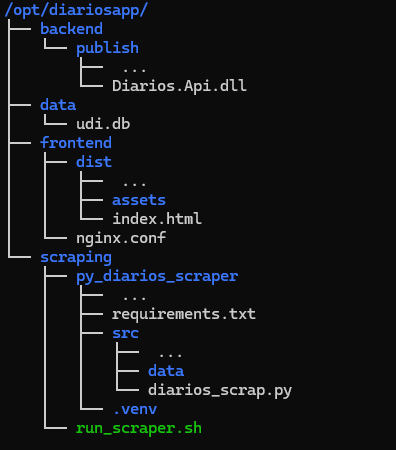
\includegraphics[width=0.6\linewidth]{figs//prints/estruturaServidorTCC.png}
    \caption{Estrutura de Diretórios no servidor}
    \label{fig:prints_estrutura_server}
\end{figure}

\subsection{Guia de Contribuições (se aplicável)}
...


%---------------------------------------------------------------------------
\section{Resultados Alcançados com o Sistema}
...

%---------------------------------------------------------------------------
\section{Considerações Sobre o Capítulo}
...
%<Neste item deve ser apresentado as considerações sobre o capítulo, incluindo uma avaliação do que fio apresentado.>